
The given equation can be written as:
\begin{align}
-x^2-xy+6y^2+30y+36=0 \label{eq:solutions/13/1/eq1}
\end{align}
\mydet{\vec{V}&\vec{u}\\\vec{u}^T&f} of \eqref{eq:solutions/13/1/eq1} becomes
\begin{align}
    \mydet{-1&-\frac{1}{2}&0\\\frac{-1}{2}&6&15\\0&15&36}=0\label{eq:solutions/13/1/eq02}
\end{align}
Expanding equation \eqref{eq:solutions/13/1/eq02}, we get zero.\\
Hence given equation represents a pair of straight lines.

The general equation second degree is given by
\begin{equation}\label{eq:solutions/13/1/eq5}
	ax^2 + 2bxy + cy^2 + 2dx + 2ey + f = 0
\end{equation}
Let $(\alpha,\beta)$ be their point of intersection, then
\begin{equation}\label{eq:solutions/13/1/eq6}
	\myvec{ a & h\\ h & b}\myvec{\alpha \\ \beta} = \myvec{-d \\ -e}
\end{equation}
Given equation is
\begin{align}
	-x^2-xy+6y^2+30y+36=0
\end{align}
Substituting in \eqref{eq:solutions/13/1/eq6}
\begin{align}
	\label{eq:solutions/13/1/eq16}\myvec{ -1 & \frac{-1}{2}\\\frac{-1}{2} & 6}\myvec{\alpha \\ \beta} = \myvec{0 \\ -15} \\
	\label{eq:solutions/13/1/eq17}\implies \myvec{\alpha \\ \beta} =\myvec{\frac{6}{5} \\ \frac{-12}{5}}
\end{align}
\text{Hence, the intersection point is}
\myvec{\frac{6}{5}\\-\frac{12}{5}}\\
Also, Verified using python code from
\begin{lstlisting}
codes/Assignment_5.py
\end{lstlisting}
From, Spectral decomposition,
\begin{align}
	\vec{V} &= \vec{P}\vec{D}\vec{P}^T\\
	\label{eq:solutions/13/1/eq18}\vec{V} &= \myvec{ -1 & \frac{-1}{2}\\\frac{-1}{2} & 6}\\
	\label{eq:solutions/13/1/eq19}\vec{P} &= \myvec{7-5 \sqrt{2} & 7+5 \sqrt{2}\\ 1 & 1}\\
	\label{eq:solutions/13/1/eq20}\vec{D} &= \myvec{\frac{5+5\sqrt{2}}{2} & 0\\ 0 & \frac{5-5\sqrt{2}}{2}}
\end{align}
P and D are also verified using python code from
\begin{lstlisting}
codes/diagonalize1.py
\end{lstlisting}
Using, \eqref{eq:solutions/13/1/eq17}, \eqref{eq:solutions/13/1/eq19} and \eqref{eq:solutions/13/1/eq20} in,
\begin{align}
	u_1(x-\alpha) + u_2(y-\beta) &= \pm \sqrt{-\frac{\lambda_2}{\lambda_1}}(v_1(x-\alpha) + v_2(y-\beta))\label{eq:solutions/13/1/eq14}
\end{align}
\begin{multline}\label{eq:solutions/13/1/eq21}
\implies	\left(7-5 \sqrt{2}\right)\left(x-\frac{30}{23}\right) + \left(y+\frac{60}{23}\right) \\= \pm \sqrt{-\frac{\frac{5-5\sqrt{2}}{2}}{\frac{5+5\sqrt{2}}{2}}}\left(\left(7-5 \sqrt{2}\right)\left(x-\frac{6}{5}\right) + \left(y+\frac{12}{5}\right)\right)
\end{multline}
simplifying \ref{eq:solutions/13/1/eq21}, we get:
\begin{align}
	\label{eq:solutions/13/1/eq22}-x + 2y + 6 = 0 \text{ and } x + 3y + 6 = 0\\
	\implies (-x + 2y + 6)(x + 3y + 6) = 0\\
	\therefore -x+2y=-6 \quad , \quad x+3y=-6\label{eq:solutions/13/1/eq23}
\end{align}


Angle between two lines, $\theta$ can be given by
\begin{align}
n_1&=(\vec{-2,-1})\\
n_2&=(\vec{-3,1})\\
\cos \theta &= \frac{\vec{n_1}^T\vec{n_2}}{\norm{\vec{n_1}}\norm{\vec{n_2}}}\\
\cos \theta&=\frac{\myvec{-2&-1}\myvec{-3\\1}}{\sqrt{(-2)^2 +(-1)^2} \times \sqrt{+(-3)^2+1}}=\frac{1}{\sqrt{2}}\\
\implies \theta &= 45\degree
\end{align}
\begin{figure}[!h]
\centering
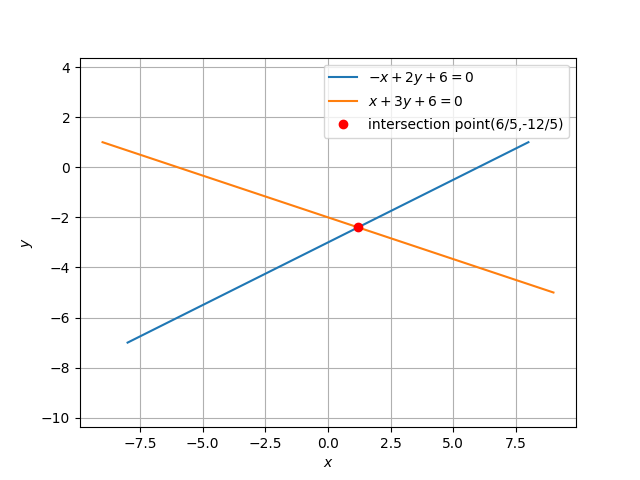
\includegraphics[width=\columnwidth]{./solutions/13/1/Figure_1.png}
\caption{plot showing intersection of lines.}
\label{eq:solutions/13/1/Fig_1}
\end{figure}
